\chapter{A Beautiful Theory}
\begin{aquote}{Murray Gell-Mann, Beauty and truth in physics, 2007}
    What is especially striking and remarkable is that in fundamental physics 
    a beautiful or elegant theory is more likely to be right 
    than a theory that is inelegant.
\end{aquote}

\section{The Standard Model}
Put simply, the Standard Model attempts to describe, at the most fundamental level, what the universe is made of and how it operates. 
So far, the content of the model is as follows: the universe is made of fermions (quarks and leptons), and it operates through the exchange of bosons (photons, gluons, W, Z, and H). 
That is, matter\footnotemark{} is composed of assemblies of fermions, which are held together, pushed apart, and otherwise interact via the fundamental forces ``transmitted'' by bosons. 
\footnotetext{With the notable exception of ``dark'' matter, which is discussed later in this chapter.}
The first and most familiar of these is the electromagnetic (EM) force because its carrier, the photon, is absorbed by the retinas in our eyes, enabling the fortunate majority of us with the gift of sight. 
Then, there is the weak force, carried by the W and Z bosons, which is responsible for the radioactive decay of certain elements. 
These first two forces are, today, understood to be unified into the ``electroweak'' (EW) force. 
Finally, there is the strong force, which holds the nuclei of atoms together. 
Alongside the forces, there is the Higgs mechanism, carried by the Higgs boson, which is responsible for giving the fundamental particles mass. 
Together, these forces and the Higgs mechanism---and gravity, whose omission here is left as a topic for another time---describe how \textit{everything} came to be and continues to be: from the sight of the sun in the sky, to the fusion reaction causing the sun to shine, to the formation of the sun and all of the other stars in the universe, to the first instance of creation itself. 
The entire universe is, we believe, the emergent motion from an elegant, infinite dance of fundamental particles. 

Of course, a stack of textbooks underlie the text above.
The concepts of fermions and bosons carry deeply insightful mathematical meaning derived originally in statistical mechanics, which was developed to describe the behavior of large ensembles of microscopic objects (like gases). 
Moreover, the particle ``zoo'' has been herded into the confines of the mathematical framework called quantum field theory (QFT), wherein particles are described as excitations of quantum ``fields'' and physical laws are realized as mathematical symmetries. 
Unfortunately, four to five years of attentive instruction and rigorous study across multiple subjects---including quantum mechanics, statistical mechanics, special relativity, and a bevy of mathematical formalism---are required to even begin reading QFT textbooks, and well over a lifetime may be required to fully understand them\footnotemark{}. 
\footnotetext{Even still, paraphrasing the great Prof. Aneesh Manohar, ``all QFT textbooks are wrong.''}
The Standard Model will instead, as promised, be described here from the perspective of an experimentalist: through hastily scrawled cartoons, rough calculations, and a great deal of hand-waving that, together, at least communicate the essential features of the theory. 

\subsection{The Higgs boson}
% Give basic overview
%    - start from lagrangians
%    - describe addition of higgs term
%    - 10-year anniversary Nature papers have a good summary
% From P5:
% The Higgs boson is an extraordinary and unique particle that is connected to the most puzzling questions of particle physics, 
% including the origin of flavor, the matter-antimatter asymmetry, dark matter and dark energy, and inflation. The Higgs boson 
% differs from other particles in that it is “frozen” in the universe. And once frozen, it is called the Higgs field because it 
% permeates the universe. The field disturbs and slows down the motion of every elementary particle. The Higgs boson slows electrons 
% in atoms so that they stay within the atom instead of flying off into space. Without the Higgs boson, or field, every electron 
%
% The Higgs boson is the only known fundamental particle that has no spin angular momentum, which permits it to have unique behavior: 
% it can interact with all known matter particles and give them mass, depending on the strength of the interaction. The Higgs boson 
% also provides a novel and distinct gateway to as yet unknown particles, such as dark matter.
%
% Find sources! Otherwise, this is great
% in every atom would move at the speed of light and everything, including us, would evaporate in a nanosecond.
Because we swore to steer away from the details of QFT, we cannot define the Higgs boson and Higgs mechanism completely. 
For this, we are better served by a primer by Griffiths~\cite{Griffiths}, followed by some QFT textbooks, and finally the original papers on the subject. % TODO: add citation for Schroeder, Schredniki, and maybe Schwartz? + Higgs papers
Instead, we will discuss it at the surface-level, starting in the classical world. 

When considering a classical system---an arrow in flight, a planet in motion, a ball on a ramp---one can describe the mechanics of that system through a Lagrangian. 
Together with the Euler-Lagrange equation, an appropriately formed Lagrangian can reproduce the ``equations of motion'' for an arbitrary system. 
The simplest example starts with the following Lagrangian $L$:
\begin{equation}
    L = \frac{1}{2}m\dot{x}^2 + U(x)
\end{equation}
where $x$ is the position of an object in just one dimension, $\dot{x}$ is the change in $x$ with respect to time (i.e. $\frac{dx}{dt}$ or the velocity) and $U(x)$ is the potential energy, which is the amount of energy needed to move an object against a certain force (e.g. $U(x) = \frac{1}{2}kx^2$ for an object fixed to a spring). 

\subsection{Feynman diagrams}
Fortunately, there is way to encode essential Standard Model calculations in a simple drawing, so-called ``Feynman diagrams,'' which, consequently, help experimentalists keep track of physically allowed processes. 
In these pictures, time flows from left to right, while space is abstractly represented on the vertical axis\footnotemark{}. 
\footnotetext{In some dark corners of the physics community, these axes are switched, but this dissertation will not deviate from the configuration described here.}
The fundamental particles are represented by lines, and the intersections of three or four of these lines (Fig.~\ref{fig:sm_vertices}) represent interactions between the corresponding particles, so at least one of them must be a boson. 
For example, an electron emitting a photon (Fig.~\ref{fig:qed1}) is represented by an electron coming in from the left, the turning into a photon and an electron leaving the picture to the right. 
This same vertex can be rotated clockwise, such that it instead depicts the annihilation of an electron and positron into a photon (Fig.~\ref{fig:ee_to_g})---one of the electrons had to be replaced with its anti-particle (a positron) to conserve charge. 
Rotating it again, we see that it now represents an electron absorbing a photon (Fig.~\ref{fig:eg_to_e}). 
These vertices act as building blocks that can be rotated and fit together according to a set of rules that correspond to real physical laws. 
Thus, any fundamental physical process (e.g. Fig.~\ref{fig:beta_decay}) can be represented with a Feynman diagram. 
Feynman diagrams are not only a visual aid for remembering which processes are allowed, however, for they also encode precise calculations about that process which can, importantly, be verified by experiment.

\begin{figure}[htb]
    \centering
    \subfloat[]{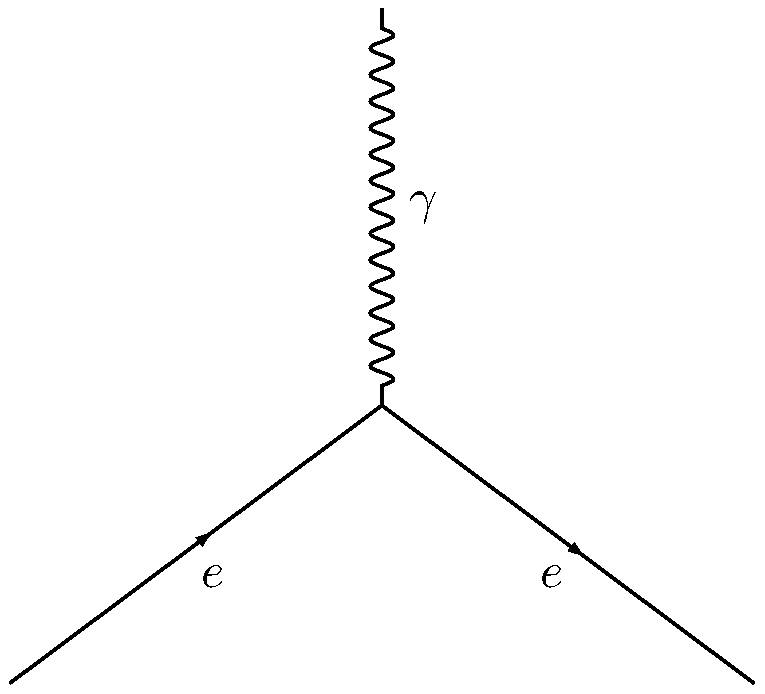
\includegraphics[width=0.25\textwidth]{fig/feynman/forces/qed_vertex.pdf}\label{fig:qed1}}\quad
    \subfloat[]{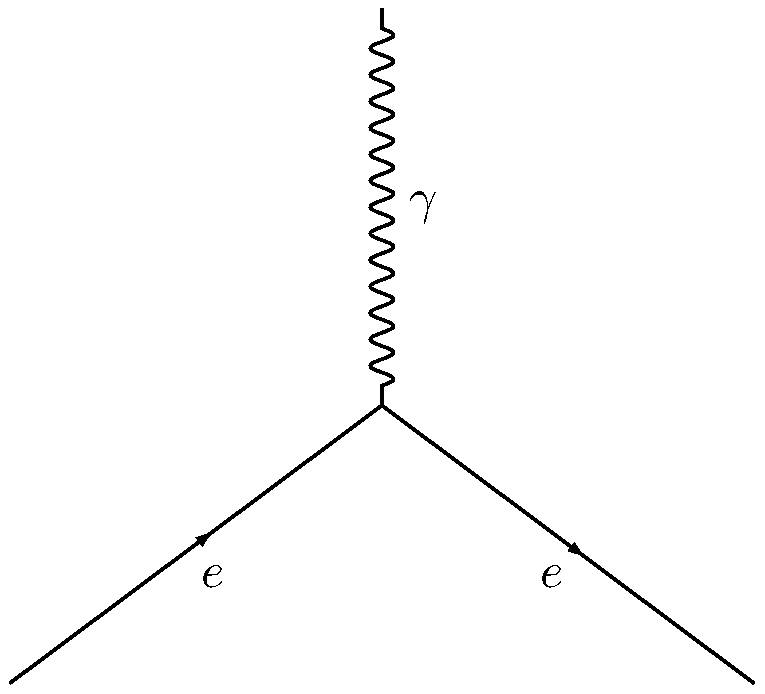
\includegraphics[width=0.25\textwidth]{fig/feynman/forces/qed_vertex.pdf}\label{fig:ewk1}}\quad
    \subfloat[]{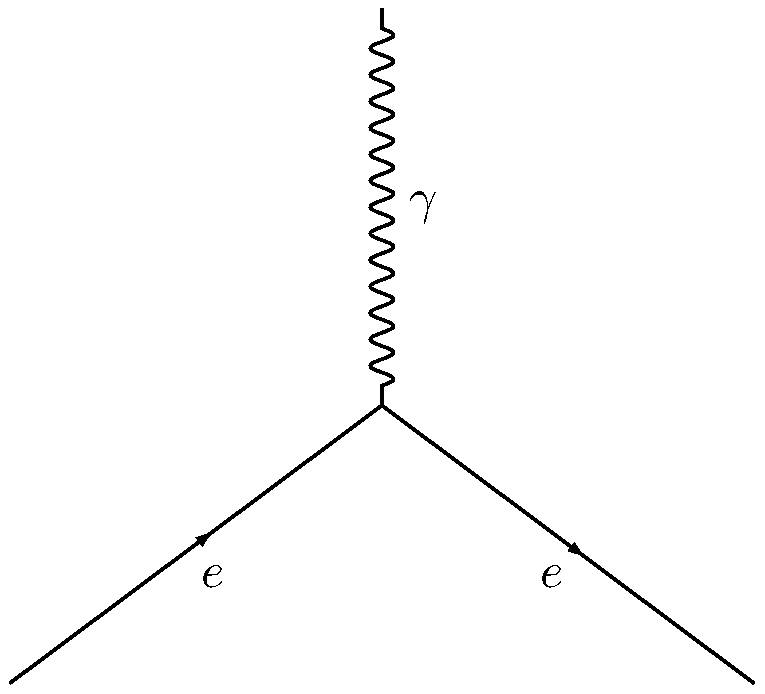
\includegraphics[width=0.25\textwidth]{fig/feynman/forces/qed_vertex.pdf}\label{fig:ewk2}}\\
    \subfloat[]{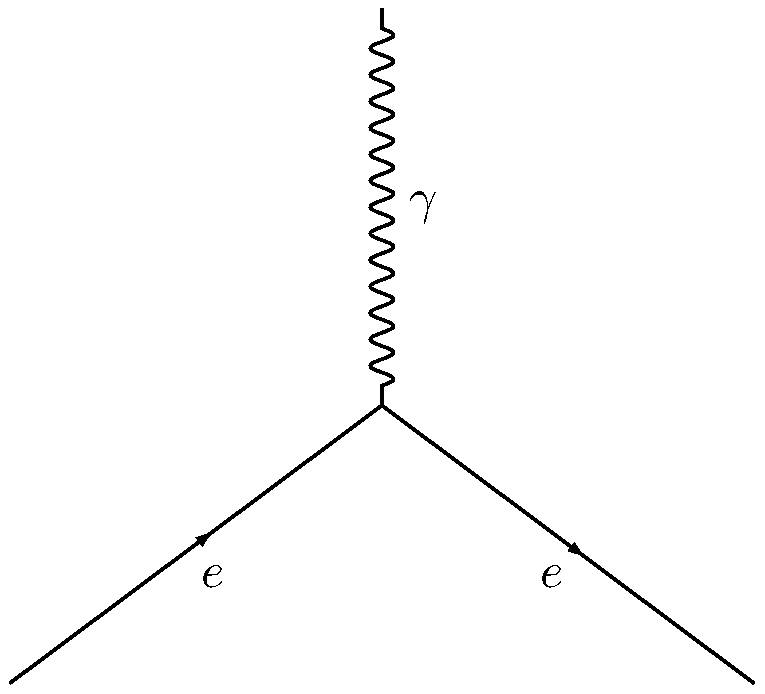
\includegraphics[width=0.25\textwidth]{fig/feynman/forces/qed_vertex.pdf}\label{fig:weak}}\quad
    \subfloat[]{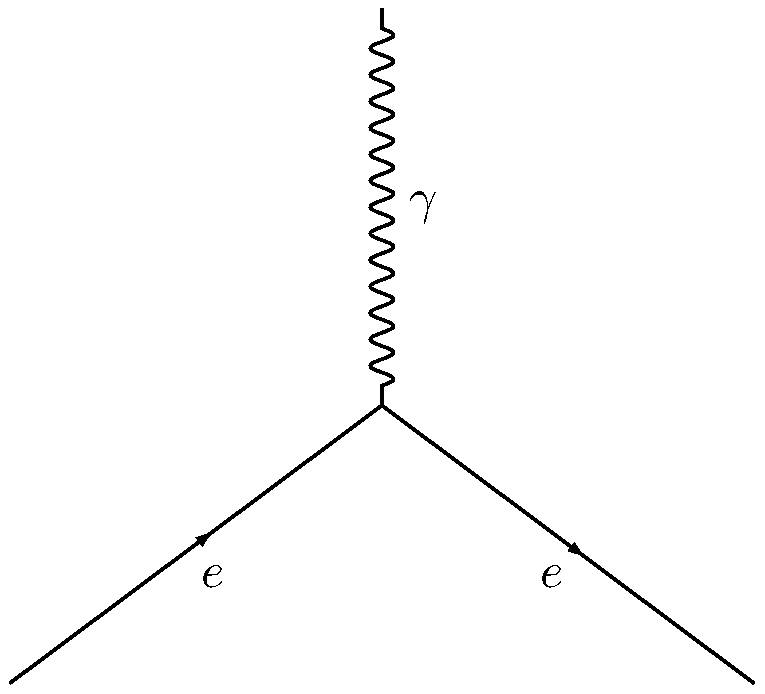
\includegraphics[width=0.25\textwidth]{fig/feynman/forces/qed_vertex.pdf}\label{fig:qcd1}}\quad
    \subfloat[]{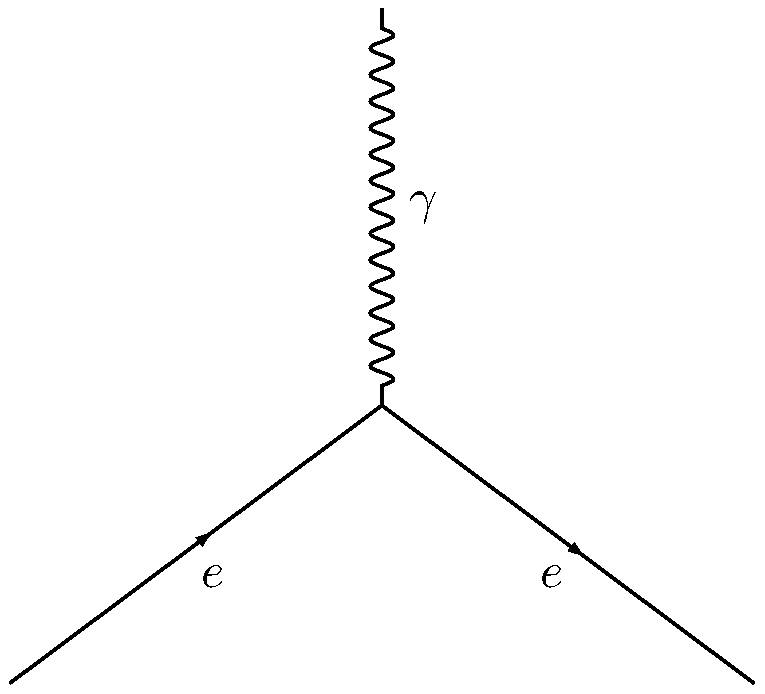
\includegraphics[width=0.25\textwidth]{fig/feynman/forces/qed_vertex.pdf}\label{fig:qcd2}}\\
    \subfloat[]{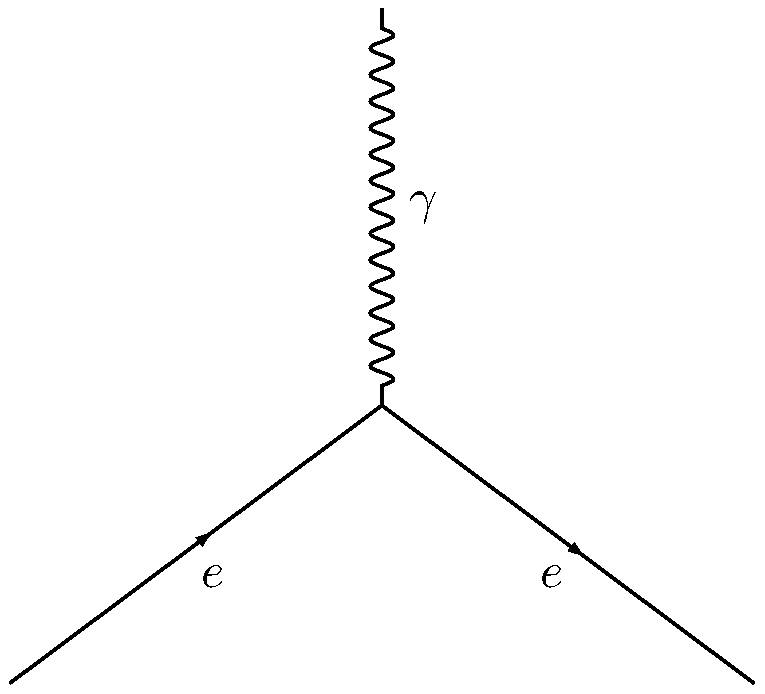
\includegraphics[width=0.25\textwidth]{fig/feynman/forces/qed_vertex.pdf}\label{fig:qcd3}}\quad
    \subfloat[]{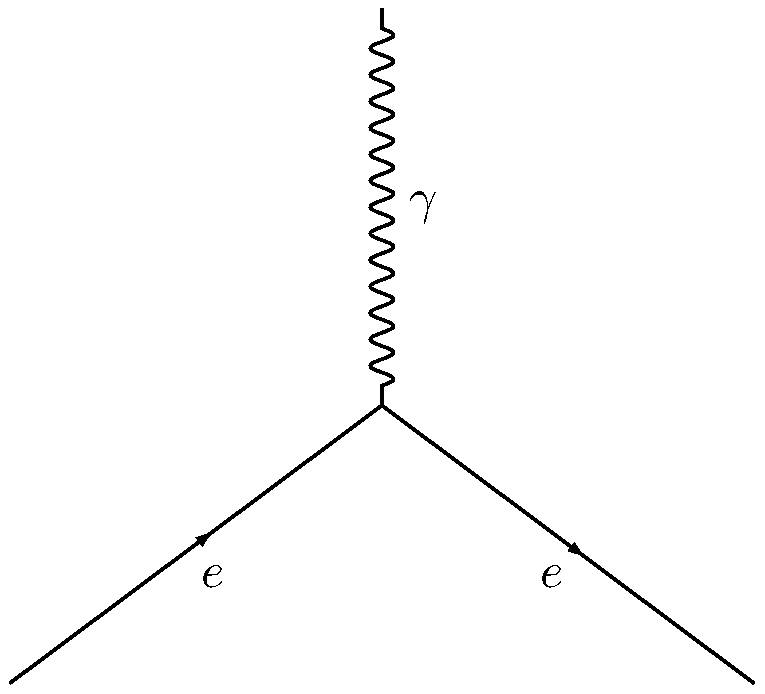
\includegraphics[width=0.25\textwidth]{fig/feynman/forces/qed_vertex.pdf}\label{fig:hig1}}\quad
    \subfloat[]{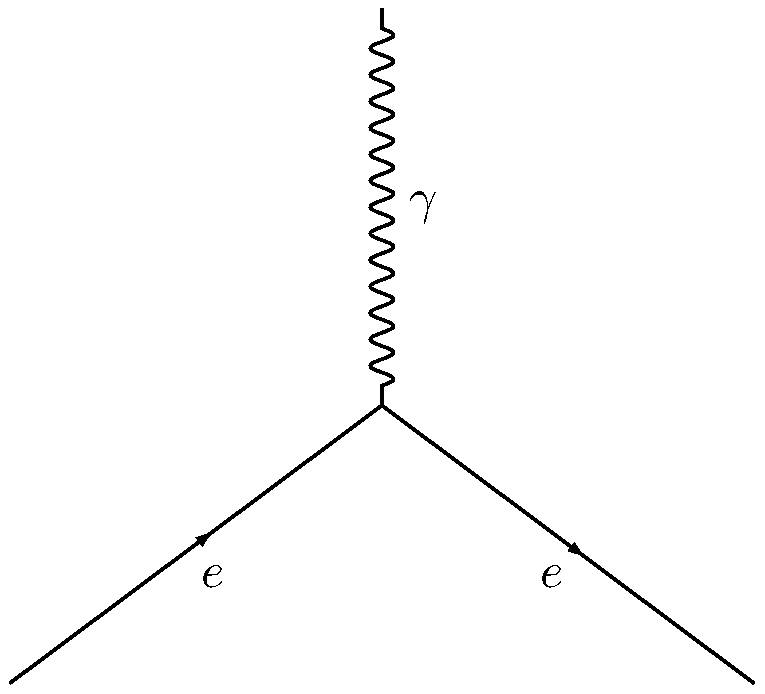
\includegraphics[width=0.25\textwidth]{fig/feynman/forces/qed_vertex.pdf}\label{fig:hig2}}
    \caption{
        The fundamental vertices in the Standard Model. 
        From left to right, top to bottom: 
        (a) electromagnetic; (b), (c) electroweak; (d) weak; (e), (f), (g) strong; (h), (i) Higgs. 
    }
    \label{fig:sm_vertices}
\end{figure}

\begin{figure}[htb]
    \centering
    \subfloat[$\Pem\to\PGg+\Pem$]{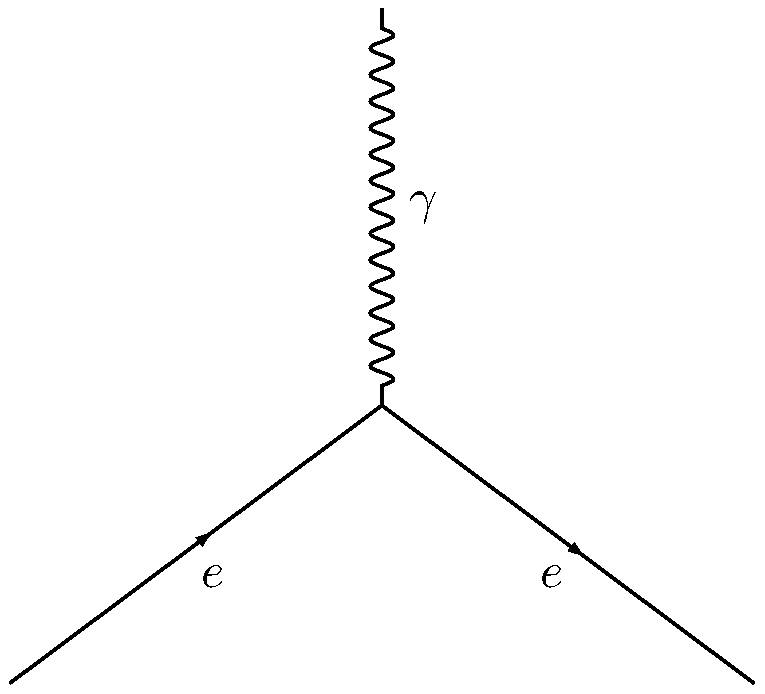
\includegraphics[width=0.25\textwidth]{fig/feynman/forces/qed_vertex.pdf}\label{fig:e_to_ge}}\quad
    \subfloat[$\Pep+\Pem\to\PGg$]{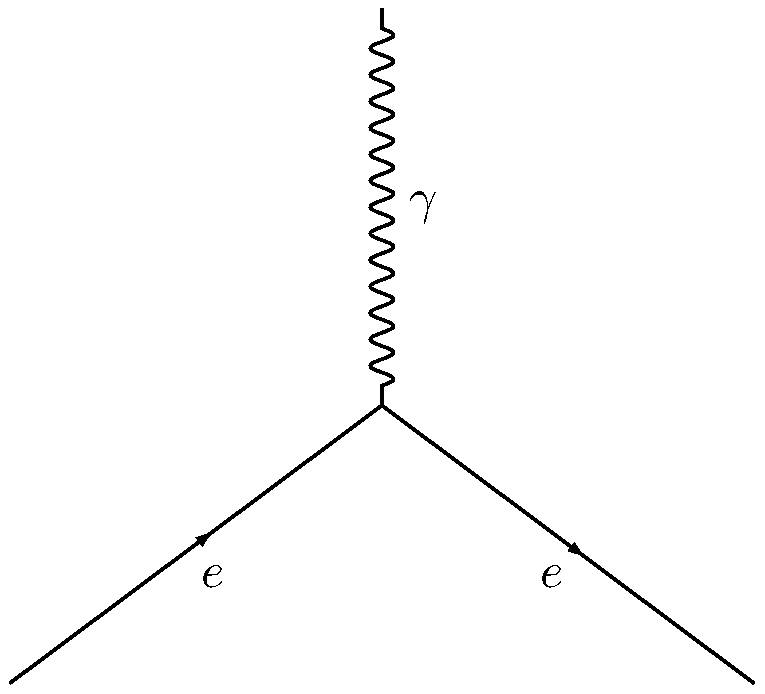
\includegraphics[width=0.25\textwidth]{fig/feynman/forces/qed_vertex.pdf}\label{fig:ee_to_g}}\quad
    \subfloat[$\Pem+\PGg\to\Pem$]{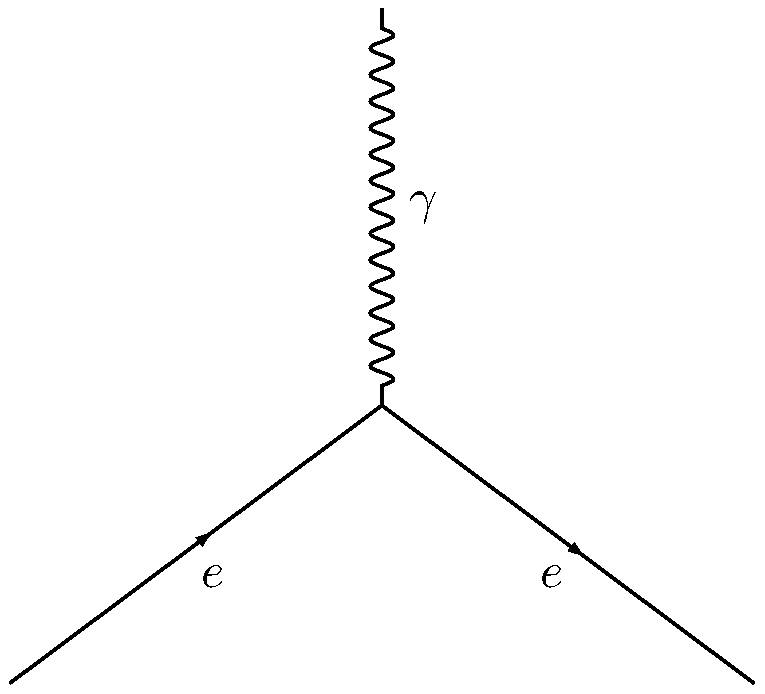
\includegraphics[width=0.25\textwidth]{fig/feynman/forces/qed_vertex.pdf}\label{fig:eg_to_e}}
    \caption{
        Rotations of the QED vertex, showing (a) an electron emitting a photon, (b) an electron and positron annihilating and producing a photon, and (c) an electron absorbing a photon. 
    }
    \label{fig:qed_rotations}
\end{figure}

\begin{figure}[htb]
    \centering
    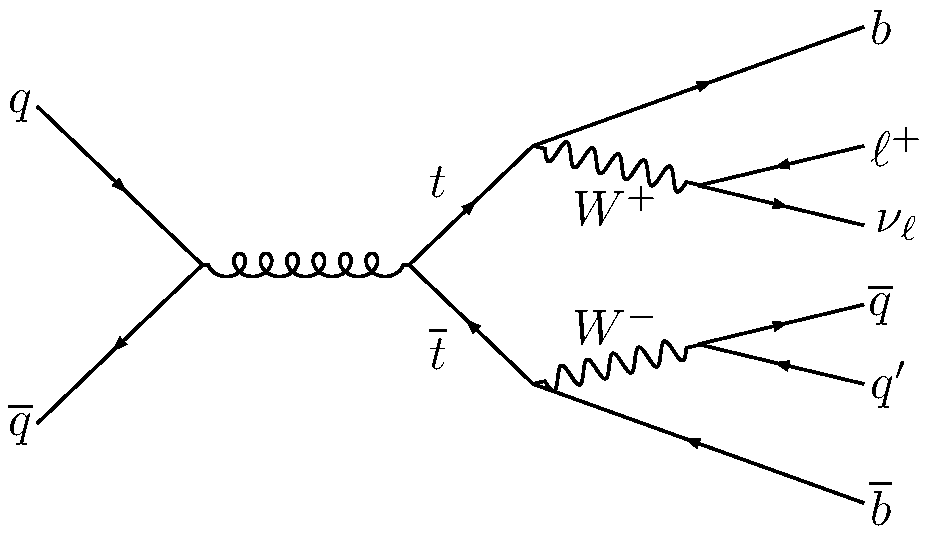
\includegraphics[width=0.6\textwidth]{fig/feynman/ttbar/ttbar_onelep.pdf} % FIXME: missing!!
    \caption{
        Feynman diagram for beta decay, which is mechanism behind the radioactive decay of certain elements. 
    }
    \label{fig:beta_decay}
\end{figure}

\subsection{Cross sections}
Consider two electrons barrelling towards each other with some velocity. 
In the classical picture, the electrons glance off one another and fly off to infinity at some angle to their original trajectories---like two errant ice skaters. 
This can be represented as a Feynman diagram (Fig.~\ref{fig:ee_scattering}) which is assembled from two EM vertices. 
Again, time flows from left to right, showing the two electrons entering, then the exchange of a photon, followed by the two electrons leaving, much like the classical picture. 
Now, suppose we construct two beams of electrons, aim them at each other, then turn them on (preferably after we leave the room). 
In this scenario, we may well want to know the probability that the two electrons will bounce off hach other (``scatter''). 
This probability is called the ``cross section,'' because it is mathematically similar to the classical picture\footnotemark{}, where we would compute the cross-sectional area presented to either of the colliding objects. 
\footnotetext{
    In fact, the answer to this question is expressed in the units of ``barns,'' literally as in ``hitting the broad side of a barn,'' coined by during World War II. % citatin needed
}
Indeed, one of the most important features of QFT is the ability to compute the cross section for scattering two electrons off of each other, as in this case, or any other interactions between particles. 
Feynman diagrams beautifully encode the complex mathematics at work here: each line and every vertex (where three lines meet) correspond a term in the calculation. 
While, again, the mathematical details are beyond the scope of this document, it is important to realize that the Feynman diagram can be directly used to calculate the cross section ($\sigma$):
\begin{equation}
    \sigma = \langle|\mathcal{M}|^2\rangle = \frac{2g_e^4}{(p_1 \cdot p_3)^2(p_1 \cdot p_4)^2[(p_1 \cdot p_2)^4 + (p_1 \cdot p_3)^4 + (p_1 \cdot p_4)^4]}
\end{equation}
where $p_1$ and $p_2$ are the four-momenta of the incoming electrons, $p_3, p_4$ are the four-momenta of the outgoing electrons, and $g_e$ is the EM coupling constant. 
This exercise, and the compact answer above, serves to demonstrate the sheer complexity of QFT calculations. 
Many details were left out beyond the computation itself (which is already a glaring omission), including details surrounding the spin of the electron, the definition of spin, the defition of four-momentum (and special relativity), and so on. 
Those details, and much more, can be found in the illustrious textbook from which this entire example was borrowed~\cite{Griffiths}. 
Moreover, this feature of QFT---the ability to compute cross sections---is absolutely vital because it offers a way of testing the theory with observation: compute the probability that the event is expected to occur, then try to reproduce that event many times in the lab and see how many times it really happens. 

\begin{figure}[htb]
    \centering
    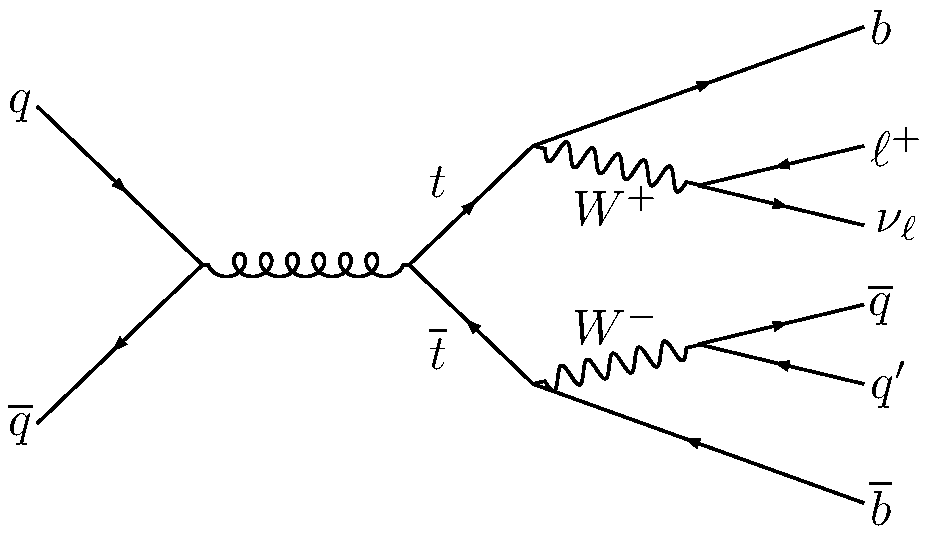
\includegraphics[width=0.6\textwidth]{fig/feynman/ttbar/ttbar_onelep.pdf} % FIXME: missing!!
    \caption{
        Feynman diagram for electron-electron scattering. 
    }
    \label{fig:ee_scattering}
\end{figure}

The validity of any model is a precarious condition: the model must exactly describe reality, else it is not a realization of the truth, but rather only approximately---or worse, accidentally---correct. 
That is, \textit{every} SM cross section value must be accurate for the validity of the model to hold. 
And so generations of physicists have made dilligent, and highly accurate, measurements of a dozens of cross sections---spanning orders of magnitude of rarity. 
Tabulated in grand tables (Fig.~\ref{fig:cms_xsecs} and \ref{fig:atlas_xsecs}), it is evident that the Standard Model has so far withstood every test derived from CMS data and ATLAS data. 
This is an incredible feat: a ``simple'' model seems to describe subatomic physics, which drove the creation of the universe and continues to drive the mechanics of everything, with incredible accuracy. 
Lingering beyond these shining trophies, however, are a number of glaring inconsistencies and enormous missing pieces. 
In other words, we know with certainty that the Standard Model is not complete, and that much more work is needed to complete it. 
We will focus in this dissertation on questions around the Higgs boson, these are detailed in the next section, because these questions motivated the bulk of the work described in the following chapters. 
However, we will also mention some additional open questions to illustrate the magnitude of the problem ahead for future particle physicists. 

\begin{figure}[htb]
    \centering
    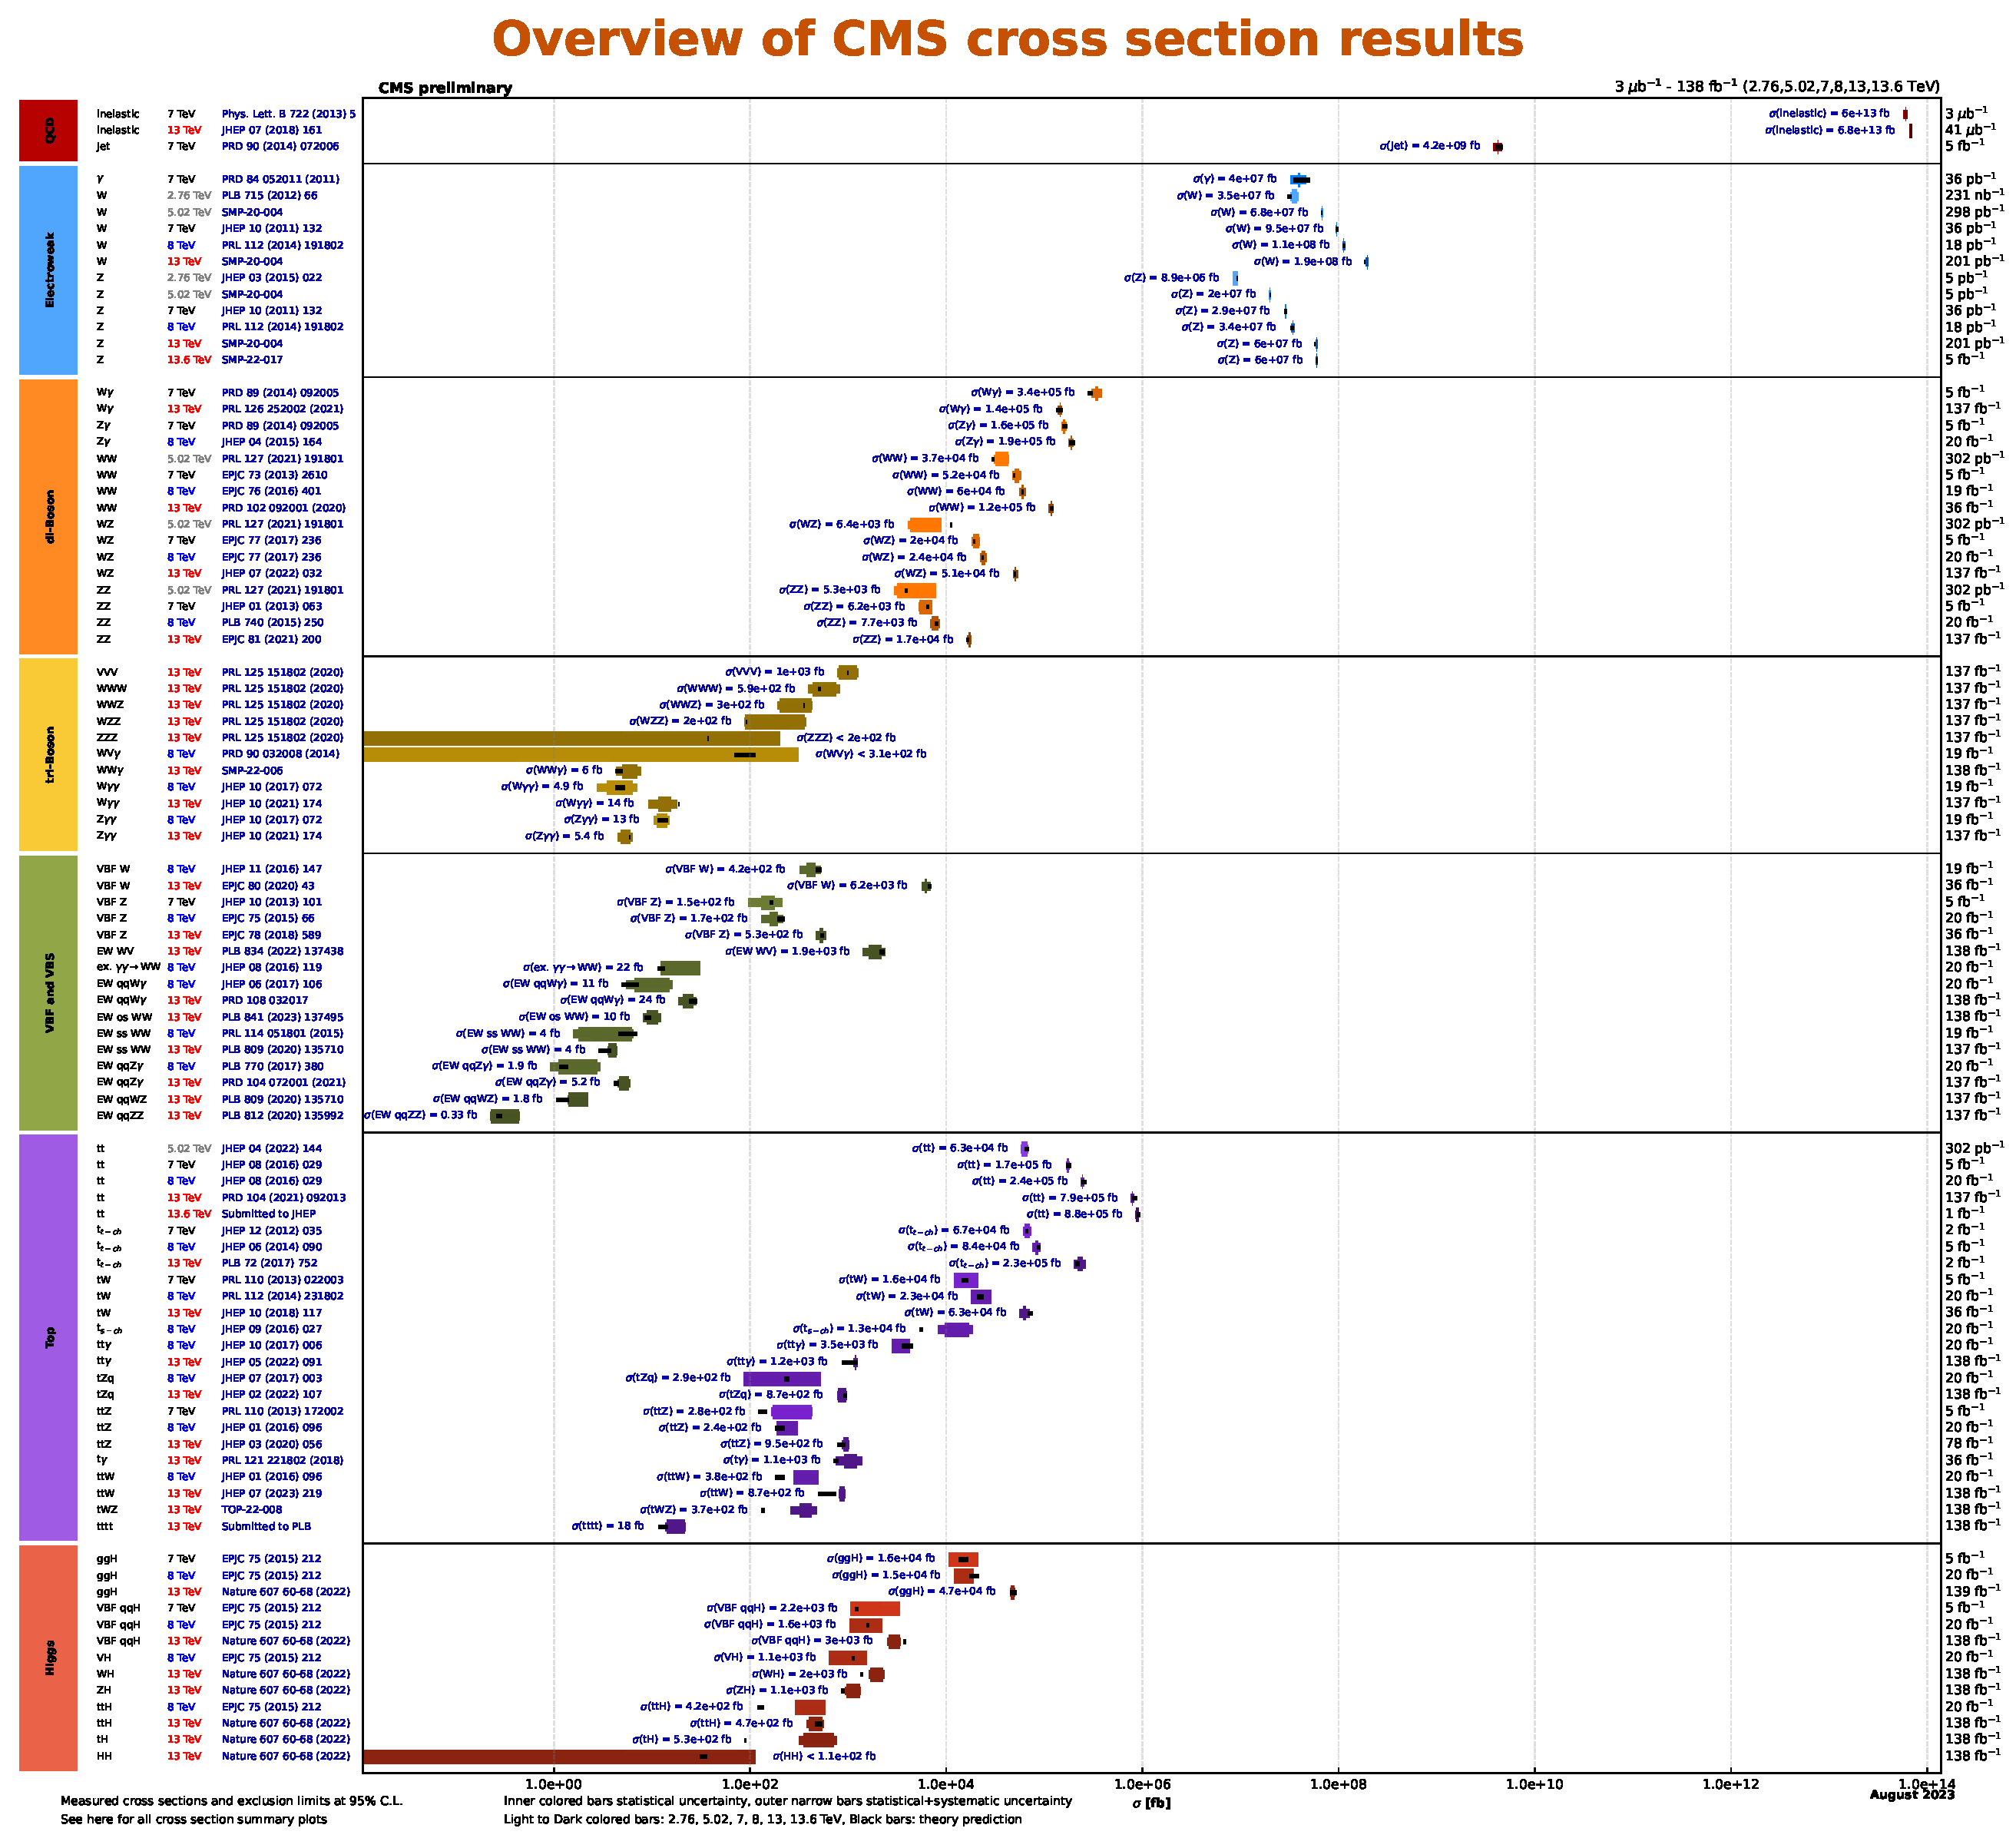
\includegraphics[width=0.9\textwidth]{fig/cms/cms_xsecs_2023.pdf}
    \caption{
        The totality of the cross section measurements performed with data from the CMS Experiment compared to the Standard Model predictions. 
        Precise agreement with the Standard Model can be seen across several orders of magnitude, representing the triumph of the model across decades of experimental scrutiny. 
        Plot taken from Ref.~\cite{CMSXSecs}.
    }
    \label{fig:cms_xsecs}
\end{figure}

\begin{figure}[htb]
    \centering
    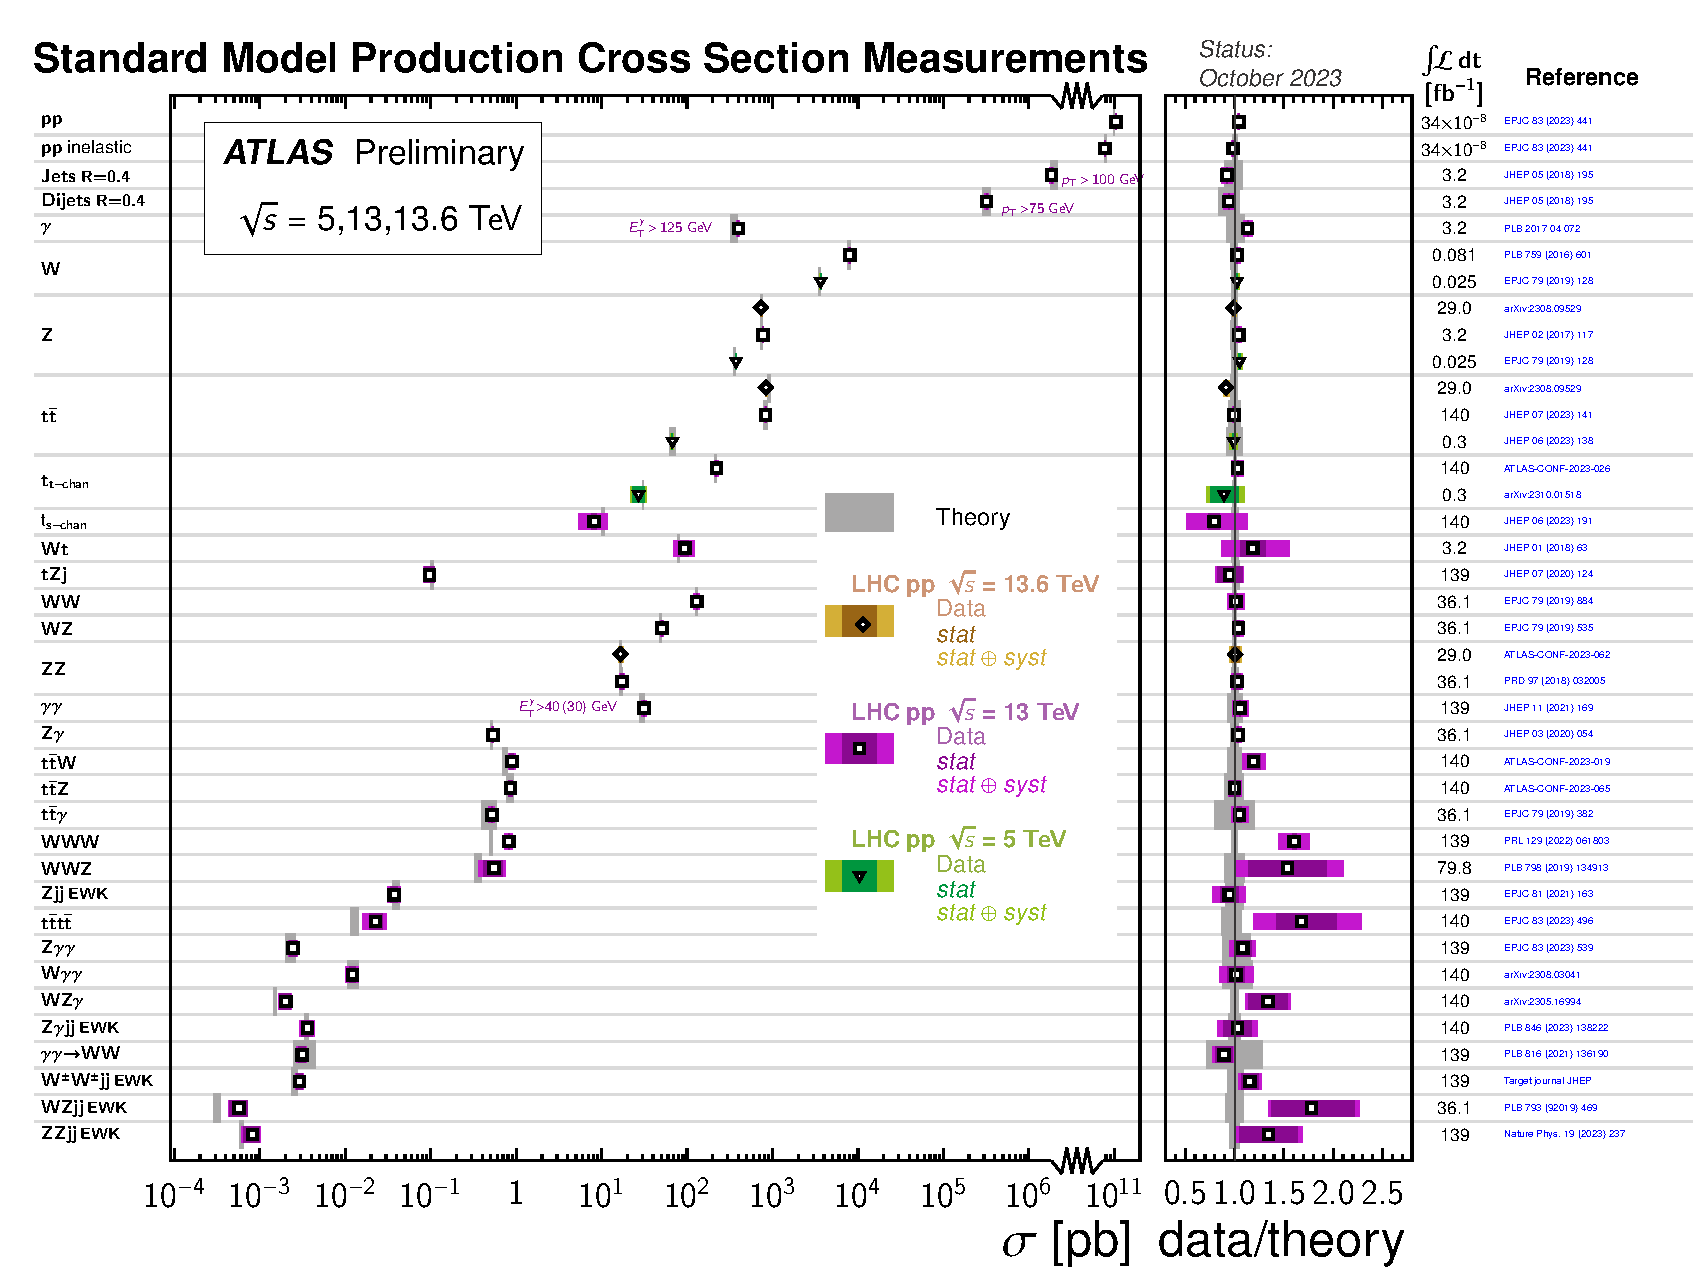
\includegraphics[width=0.9\textwidth]{fig/atlas/atlas_xsecs_2023.pdf}
    \caption{
        A selection of cross section measurements performed with data from the ATLAS Experiment compared to the Standard Model predictions. 
        Precise agreement with the Standard Model can be seen across several orders of magnitude, representing the triumph of the model across decades of experimental scrutiny. 
        Plot taken from Ref.~\cite{ATL-PHYS-PUB-2023-039}.
    }
    \label{fig:atlas_xsecs}
\end{figure}

\section{Open questions}\label{sec:open_questions}
% Higgs sector:
%    - naturalness?
%    - other higgses?? Gell-Mann said something like "it would be weird if 
%      there was only one Higgs boson" in 2012 CERN interview
%    - other problems... I guess introduce problem of not yet measuring 
%      higgs couplings well
% More generic:
%    - dark matter
